\documentclass{beamer}
\usepackage{graphics,color}
\usepackage{textcomp}
\usepackage{xcolor}
\usepackage{pgfplots}
\usepackage{pgfplotstable}
\usepackage{booktabs}
\usepackage{array}
\usepackage{colortbl}
\usepackage{amsmath,mathpazo}
\usepackage[utf8]{inputenc}
\usepackage{multicol}

\newcommand\blfootnote[1]{%
  \begingroup
  \renewcommand\thefootnote{}\footnote{#1}%
  \addtocounter{footnote}{-1}%
  \endgroup
}



\title{Buck Converter Power Train in Skywater 130nm}
\author{Teo Ene \\
  Ross Thompson}
\institute{Oklahoma State University}
\date{April 2022}

\usetheme{osu}

\begin{document}

\frame{\titlepage}

\begin{frame}
  \frametitle{Overview}
  \begin{itemize}
  \item Topology
  \item Design Parameters
  \item Circuit
  \item Deadtime
  \item Specification
  \end{itemize}
\end{frame}

\begin{frame}
  \frametitle{Topology and Design Goals}
  \begin{itemize}
  \item High efficiency voltage conversion from $3.6V$ to $1.8V$.
  \item Supply at least $400mA$.
  \item Ripple $< 40mV$
  \item Work with reasonably wide input supply $3.0$ to $4.4V$.
  \end{itemize}        
\end{frame}

\begin{frame}
  \frametitle{Passive Components and Design Selection}
  \begin{itemize}
  \item Inductor
    \begin{itemize}
    \item Inductance
    \item ESR
    \end{itemize}
  \item Capacitor
    \begin{itemize}
    \item Capacitance
    \item ESR $@ 1MHz$ $10 m\Omega$
    \end{itemize}
  \item Switching frequency $1Mhz$ (Found experimentally)
  \end{itemize}
\end{frame}

\begin{frame}
  \frametitle{Buck}
  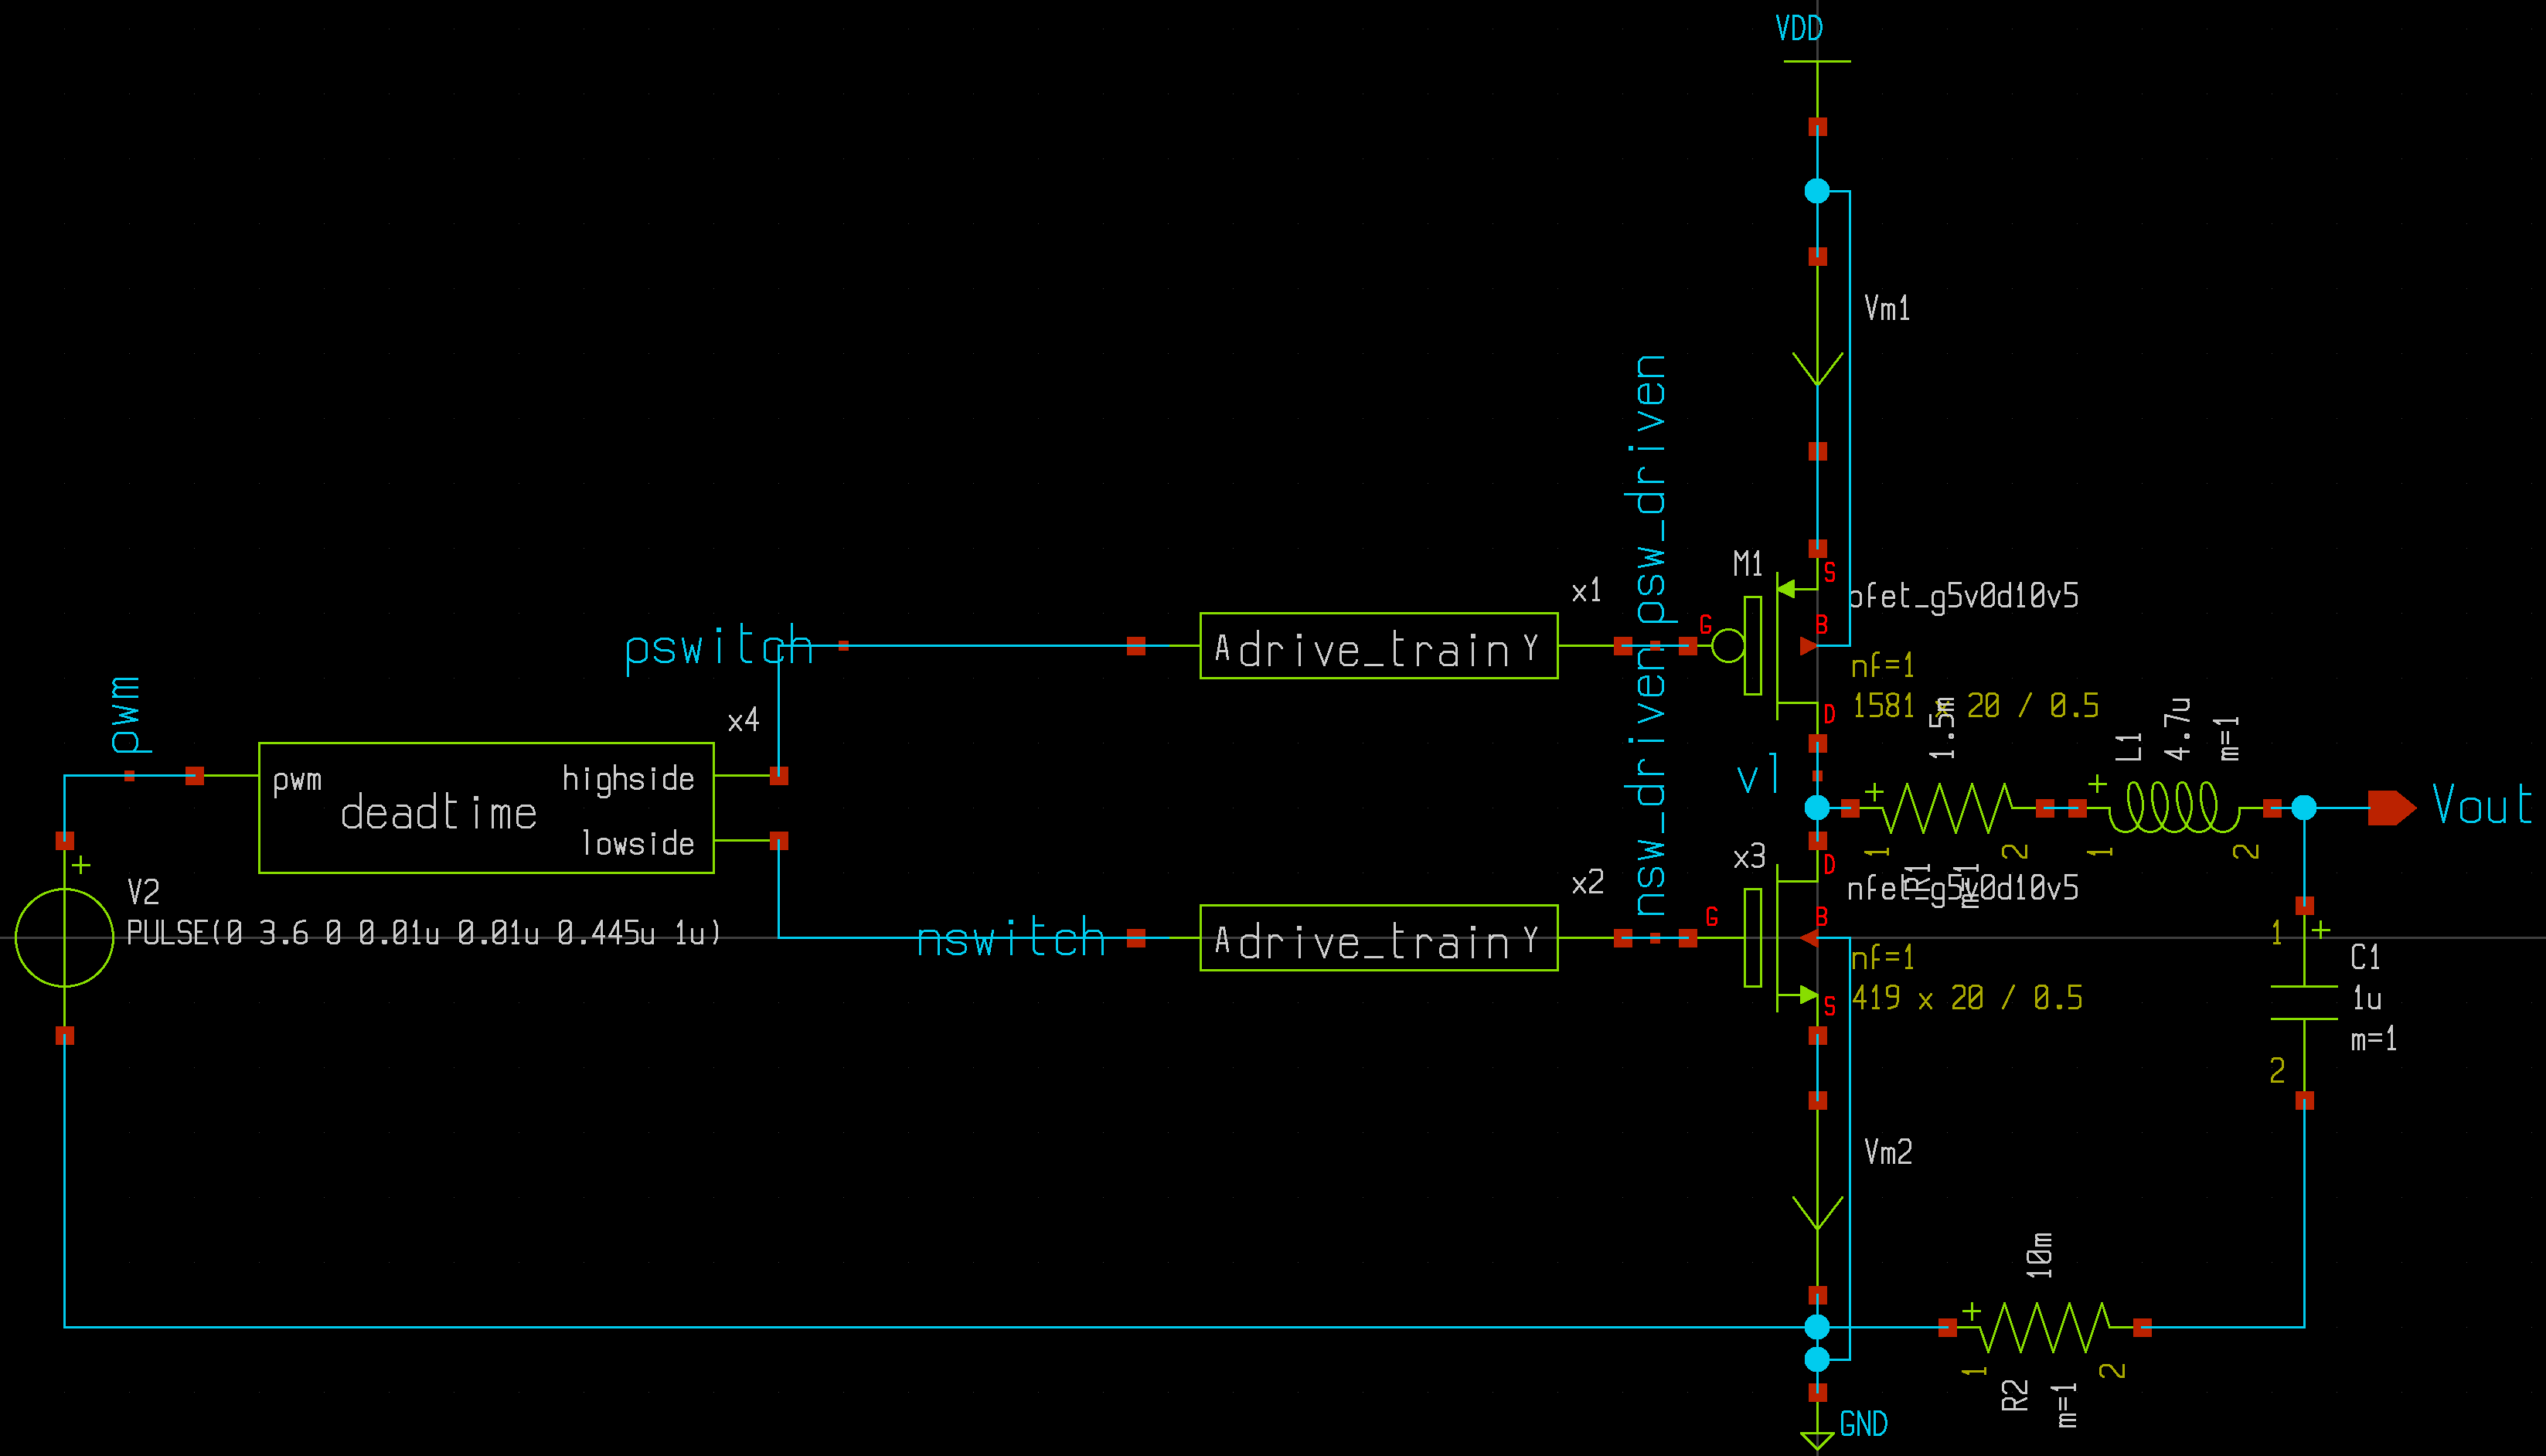
\includegraphics[scale=0.08]{buck.png}
\end{frame}

\begin{frame}
  \frametitle{Drive Train}
  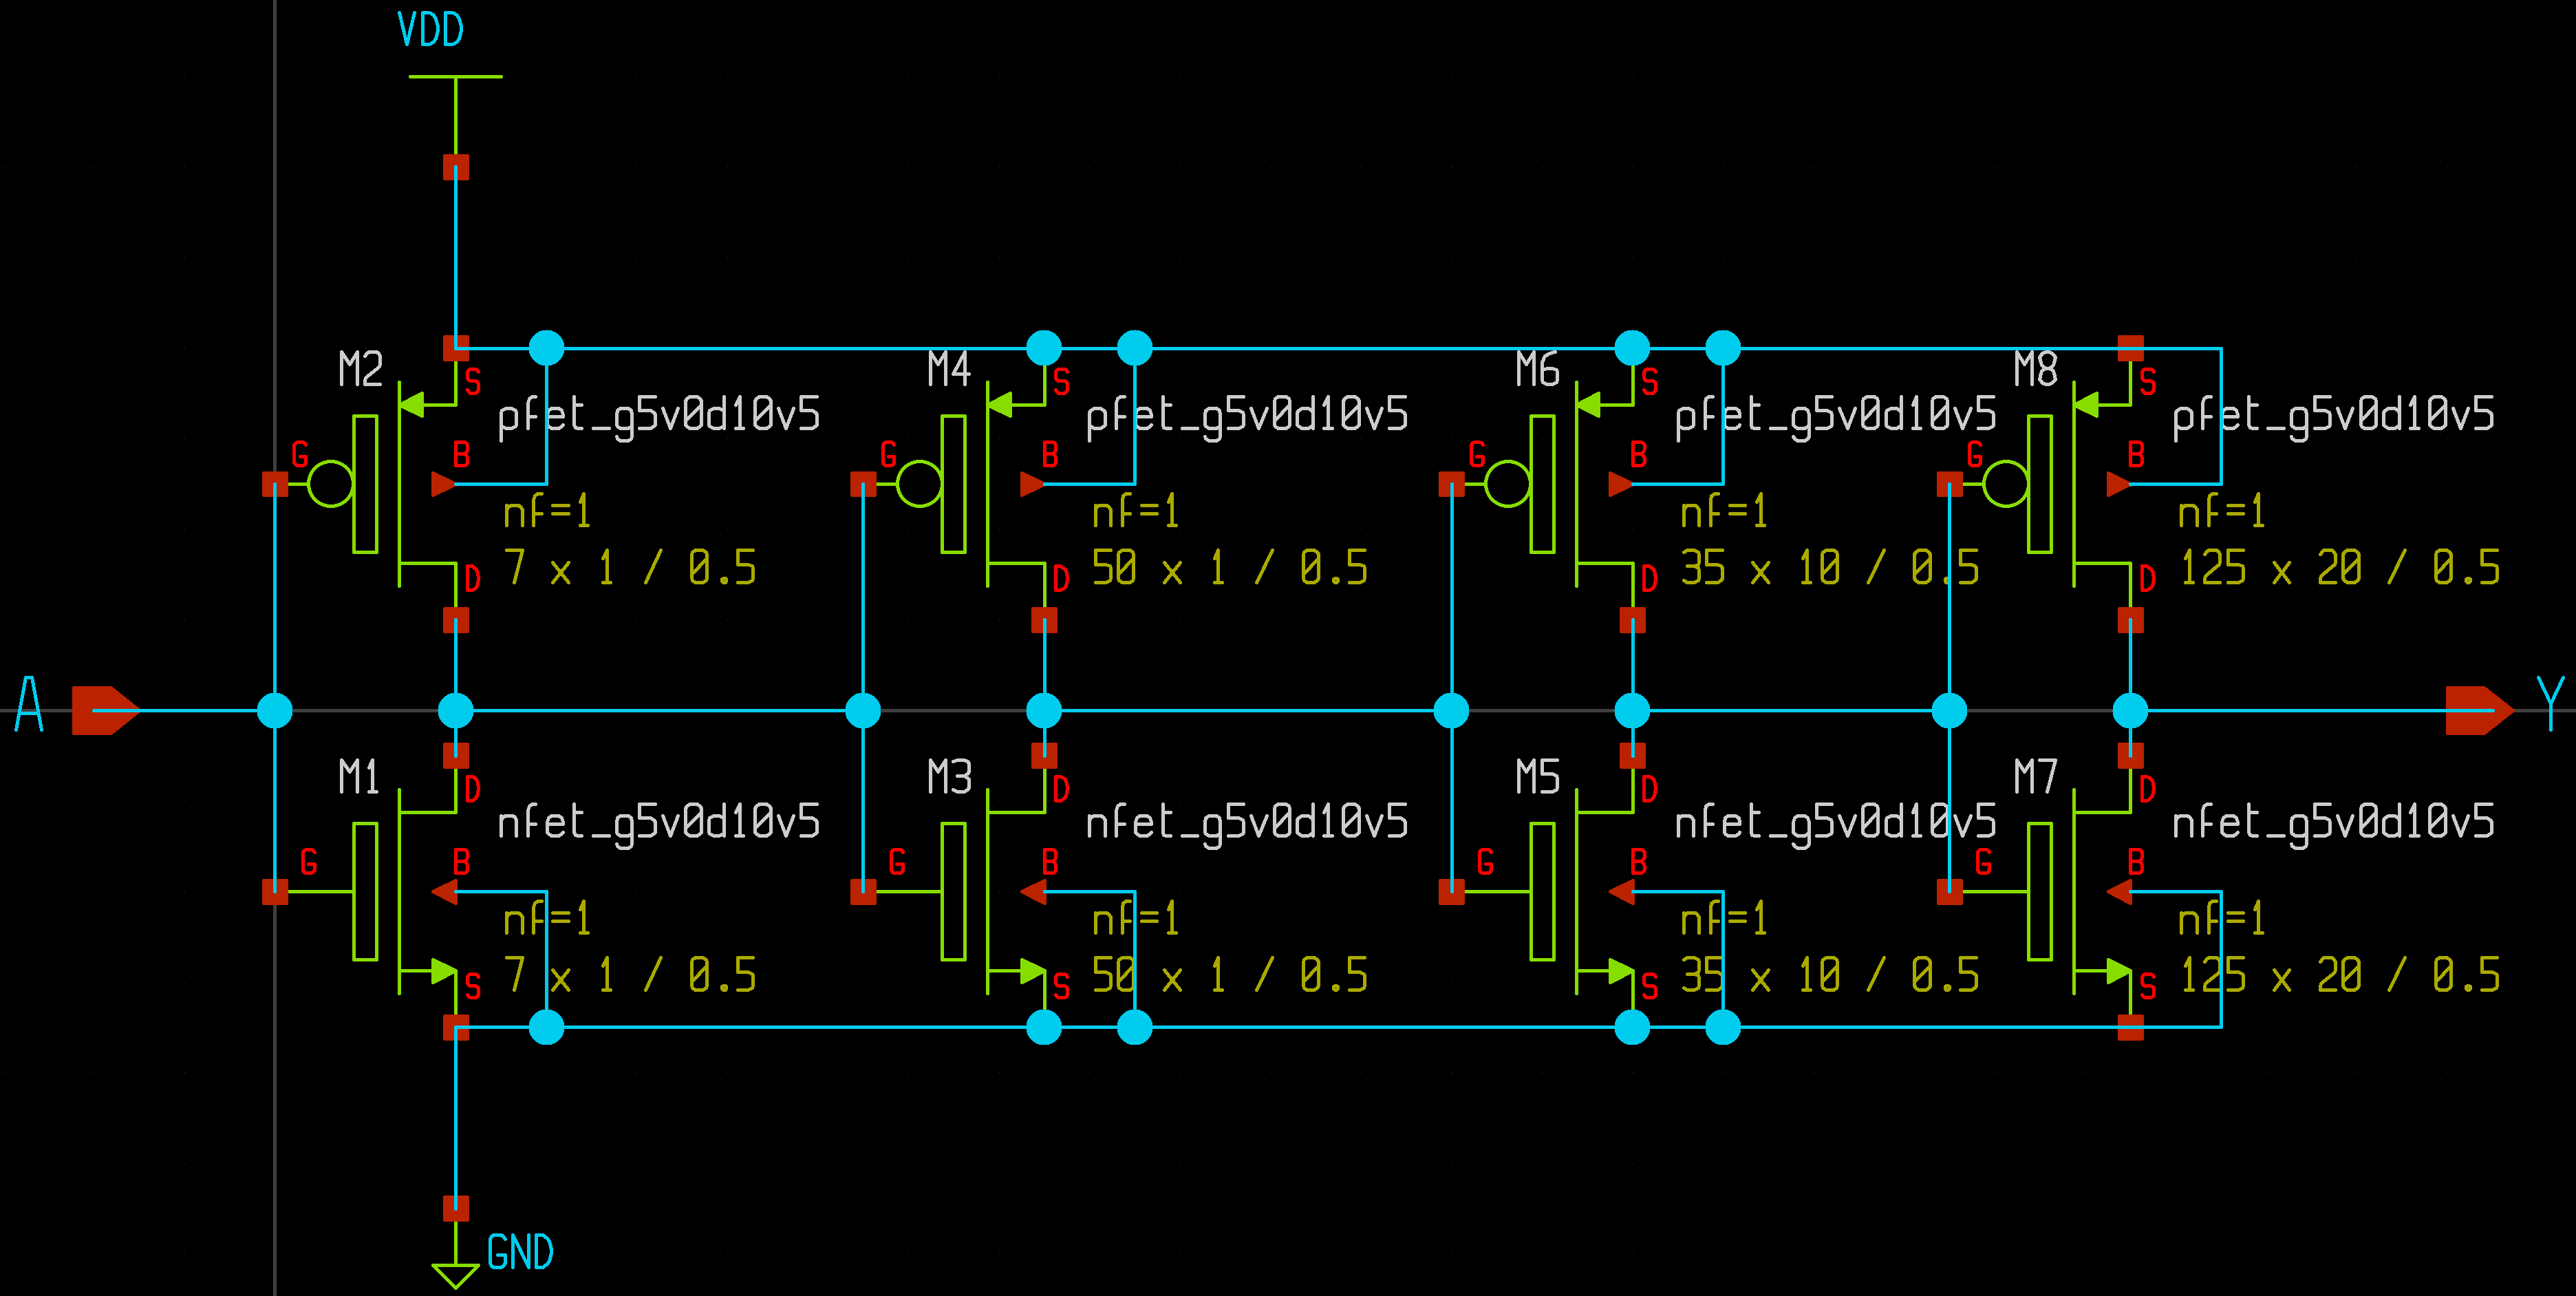
\includegraphics[scale=0.08]{drive-train.png}
\end{frame}

\begin{frame}
  \frametitle{Deadtime}
  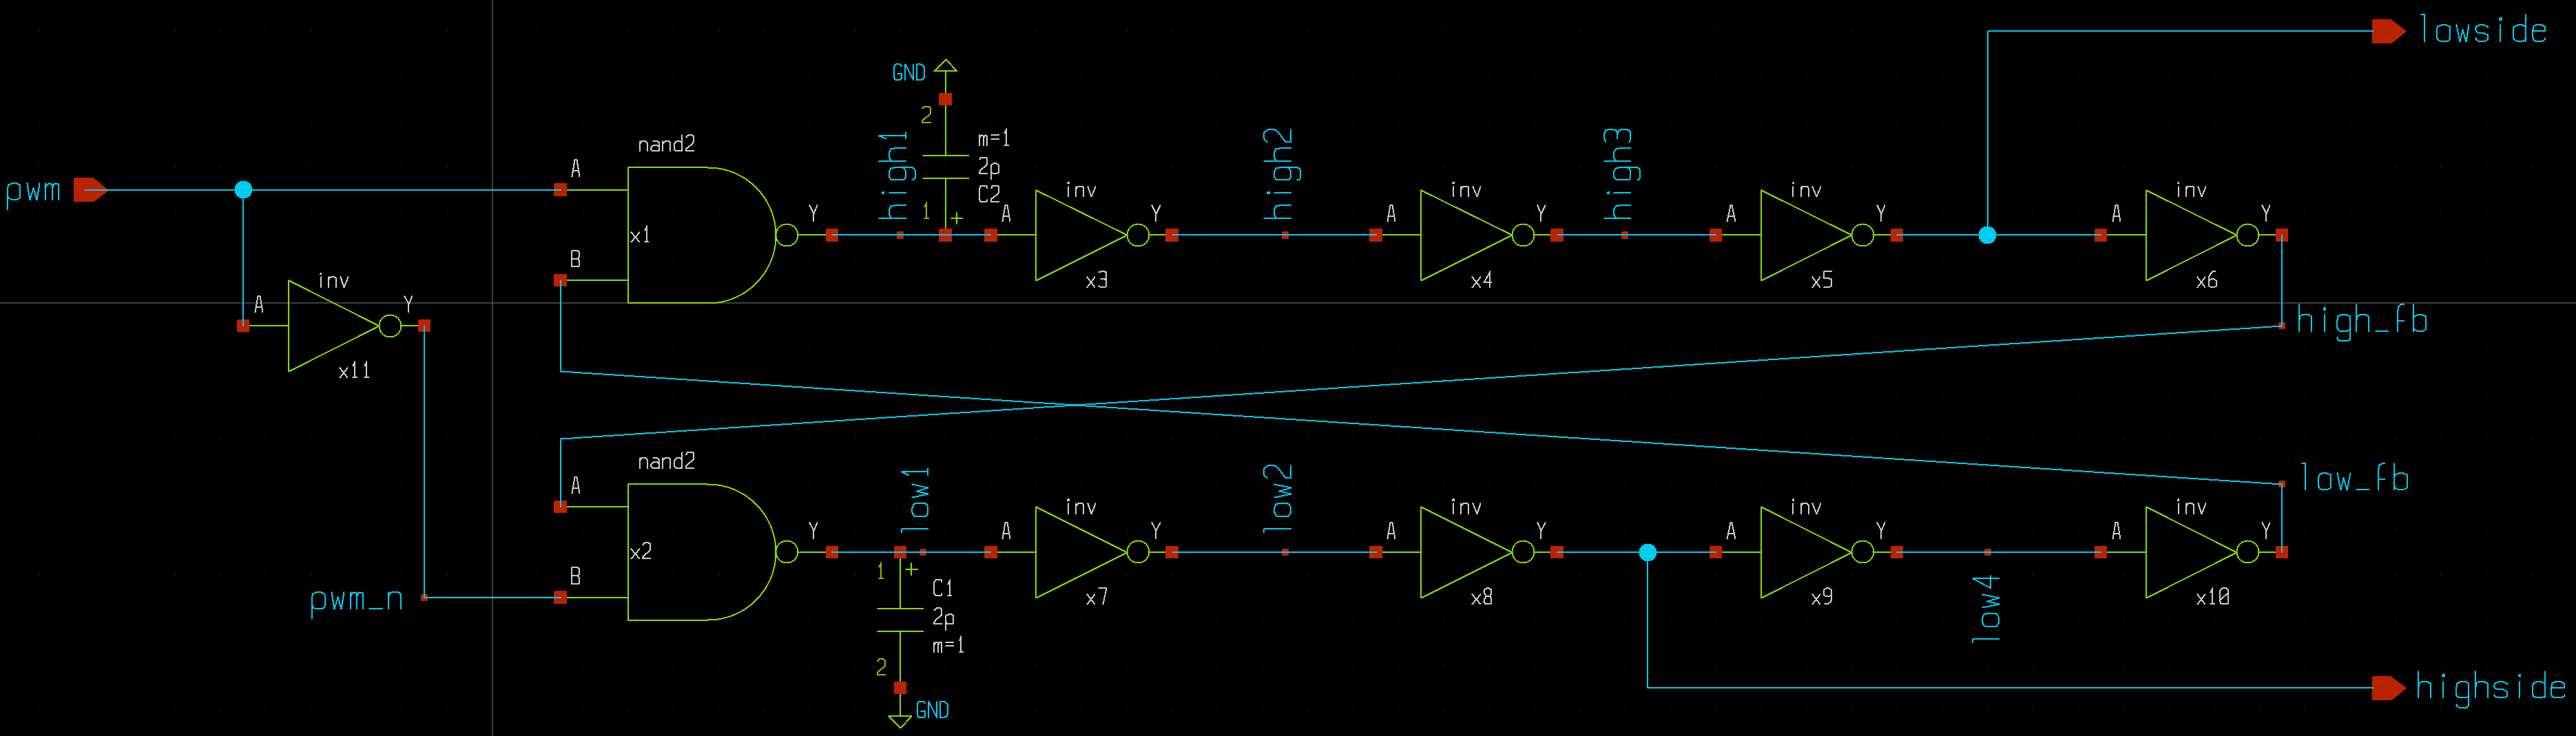
\includegraphics[scale=0.085]{deadtime.png}
  \begin{itemize}
  \item 4 chain inverter adds delay.
  \item NAND creates deadtime.
  \item 2pF cap increases propagation delay
  \item Deadtime = ~20ps or 2\%  of period
  \end{itemize}
\end{frame}

\begin{frame}
  \frametitle{Deadtime Inverter}
  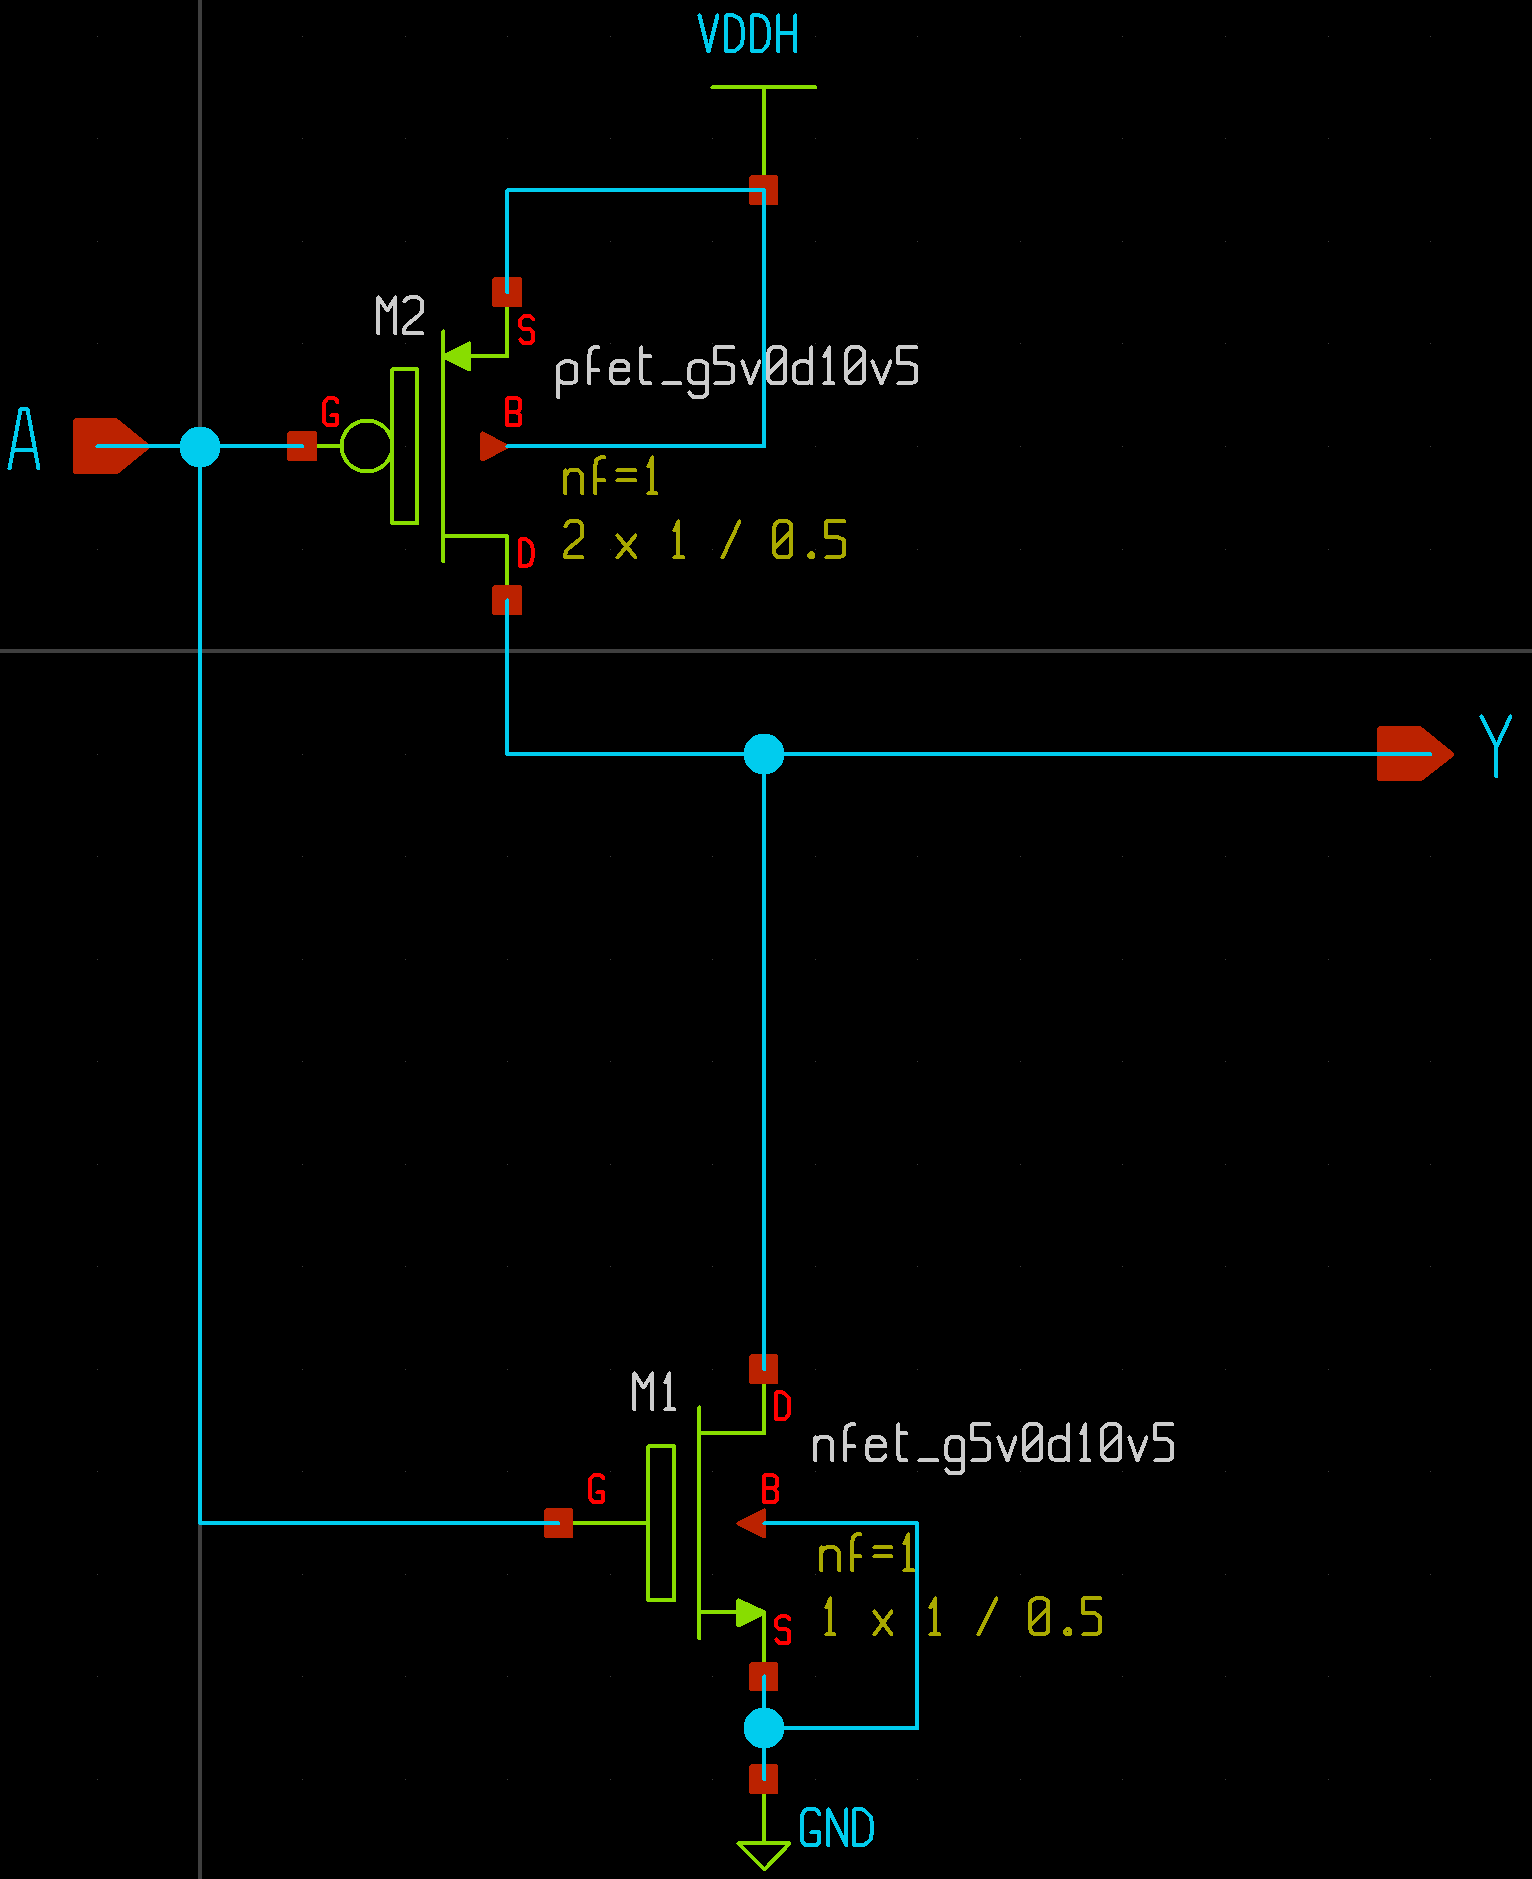
\includegraphics[scale=0.09]{inverter.png}
  \begin{itemize}
  \item Min sized 5V tolerant
  \end{itemize}
\end{frame}
\begin{frame}
  \frametitle{Deadtime NAND}
  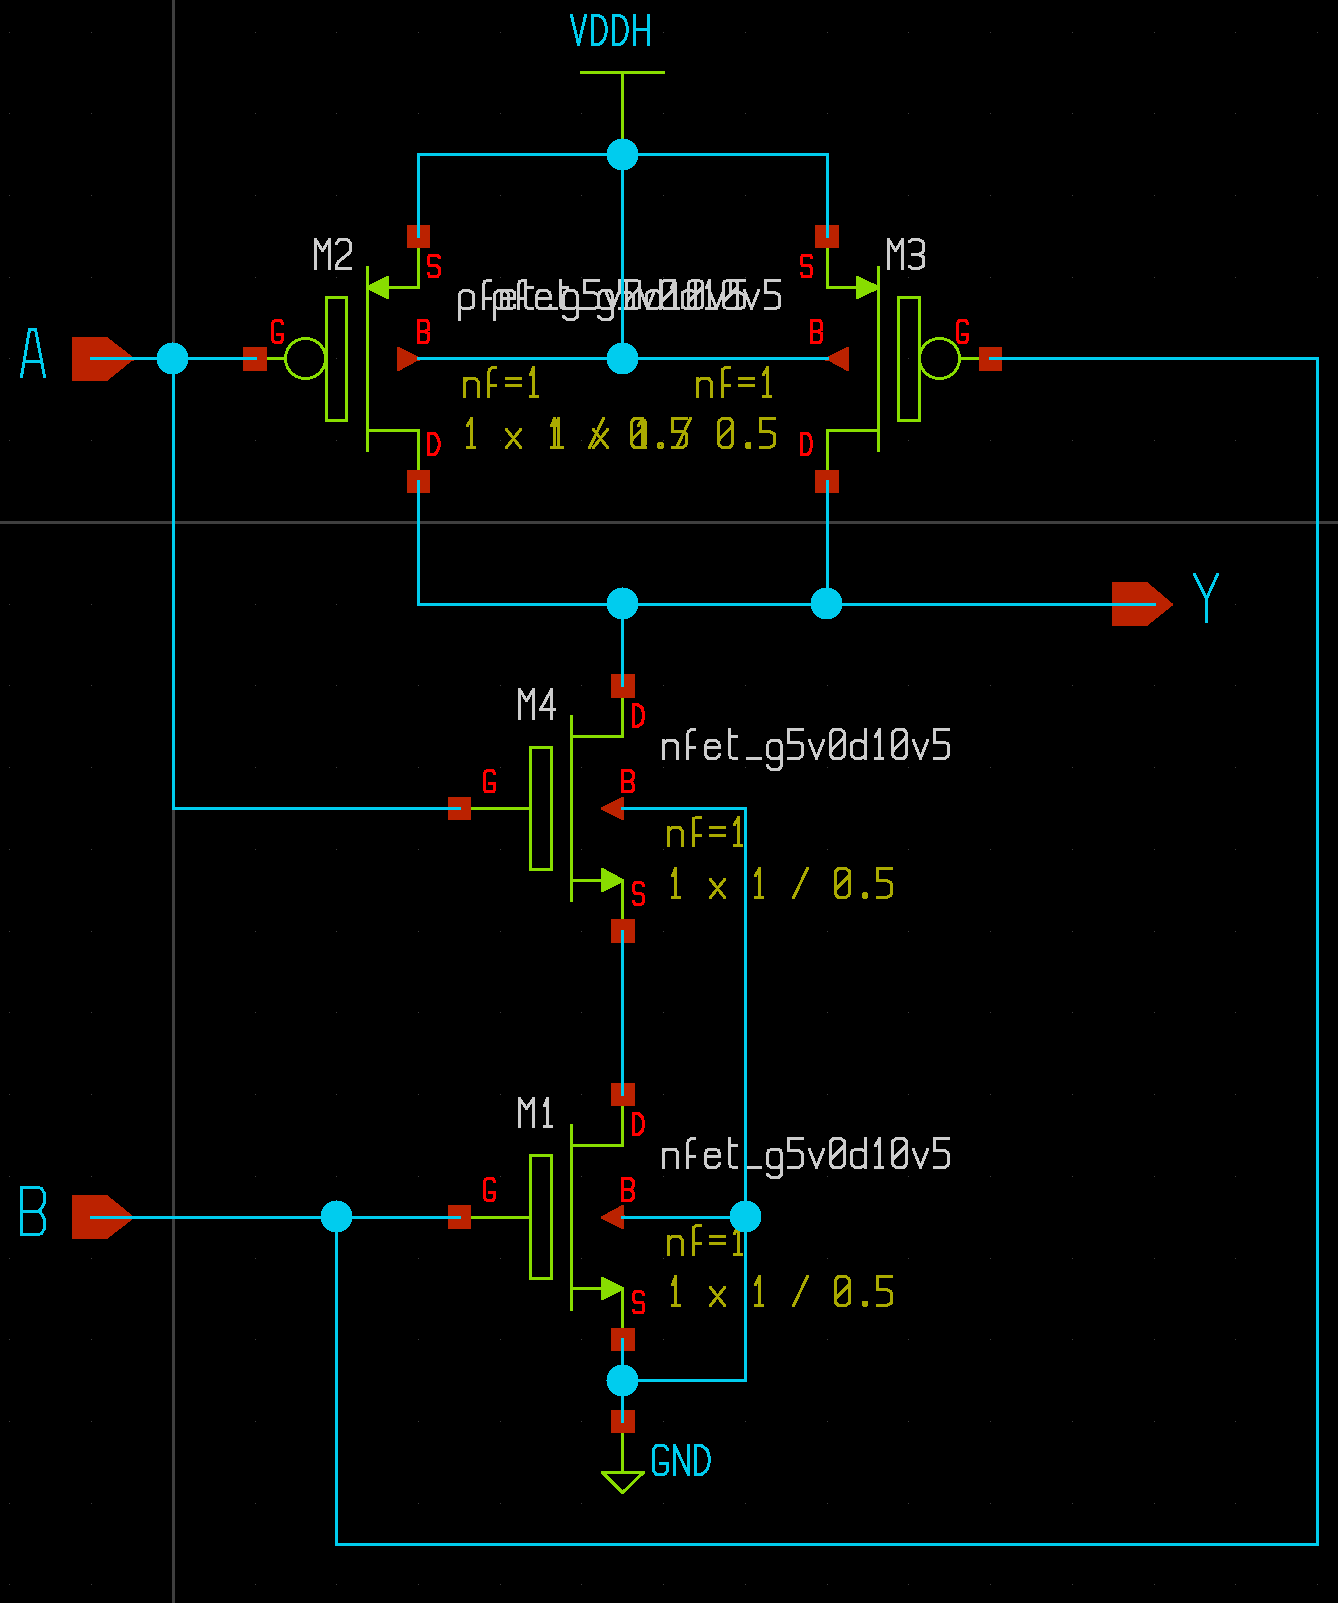
\includegraphics[scale=0.09]{nand.png}
  \begin{itemize}
  \item Min sized 5V tolerant
  \end{itemize}
\end{frame}

\begin{frame}
  \frametitle{Test Bench}
  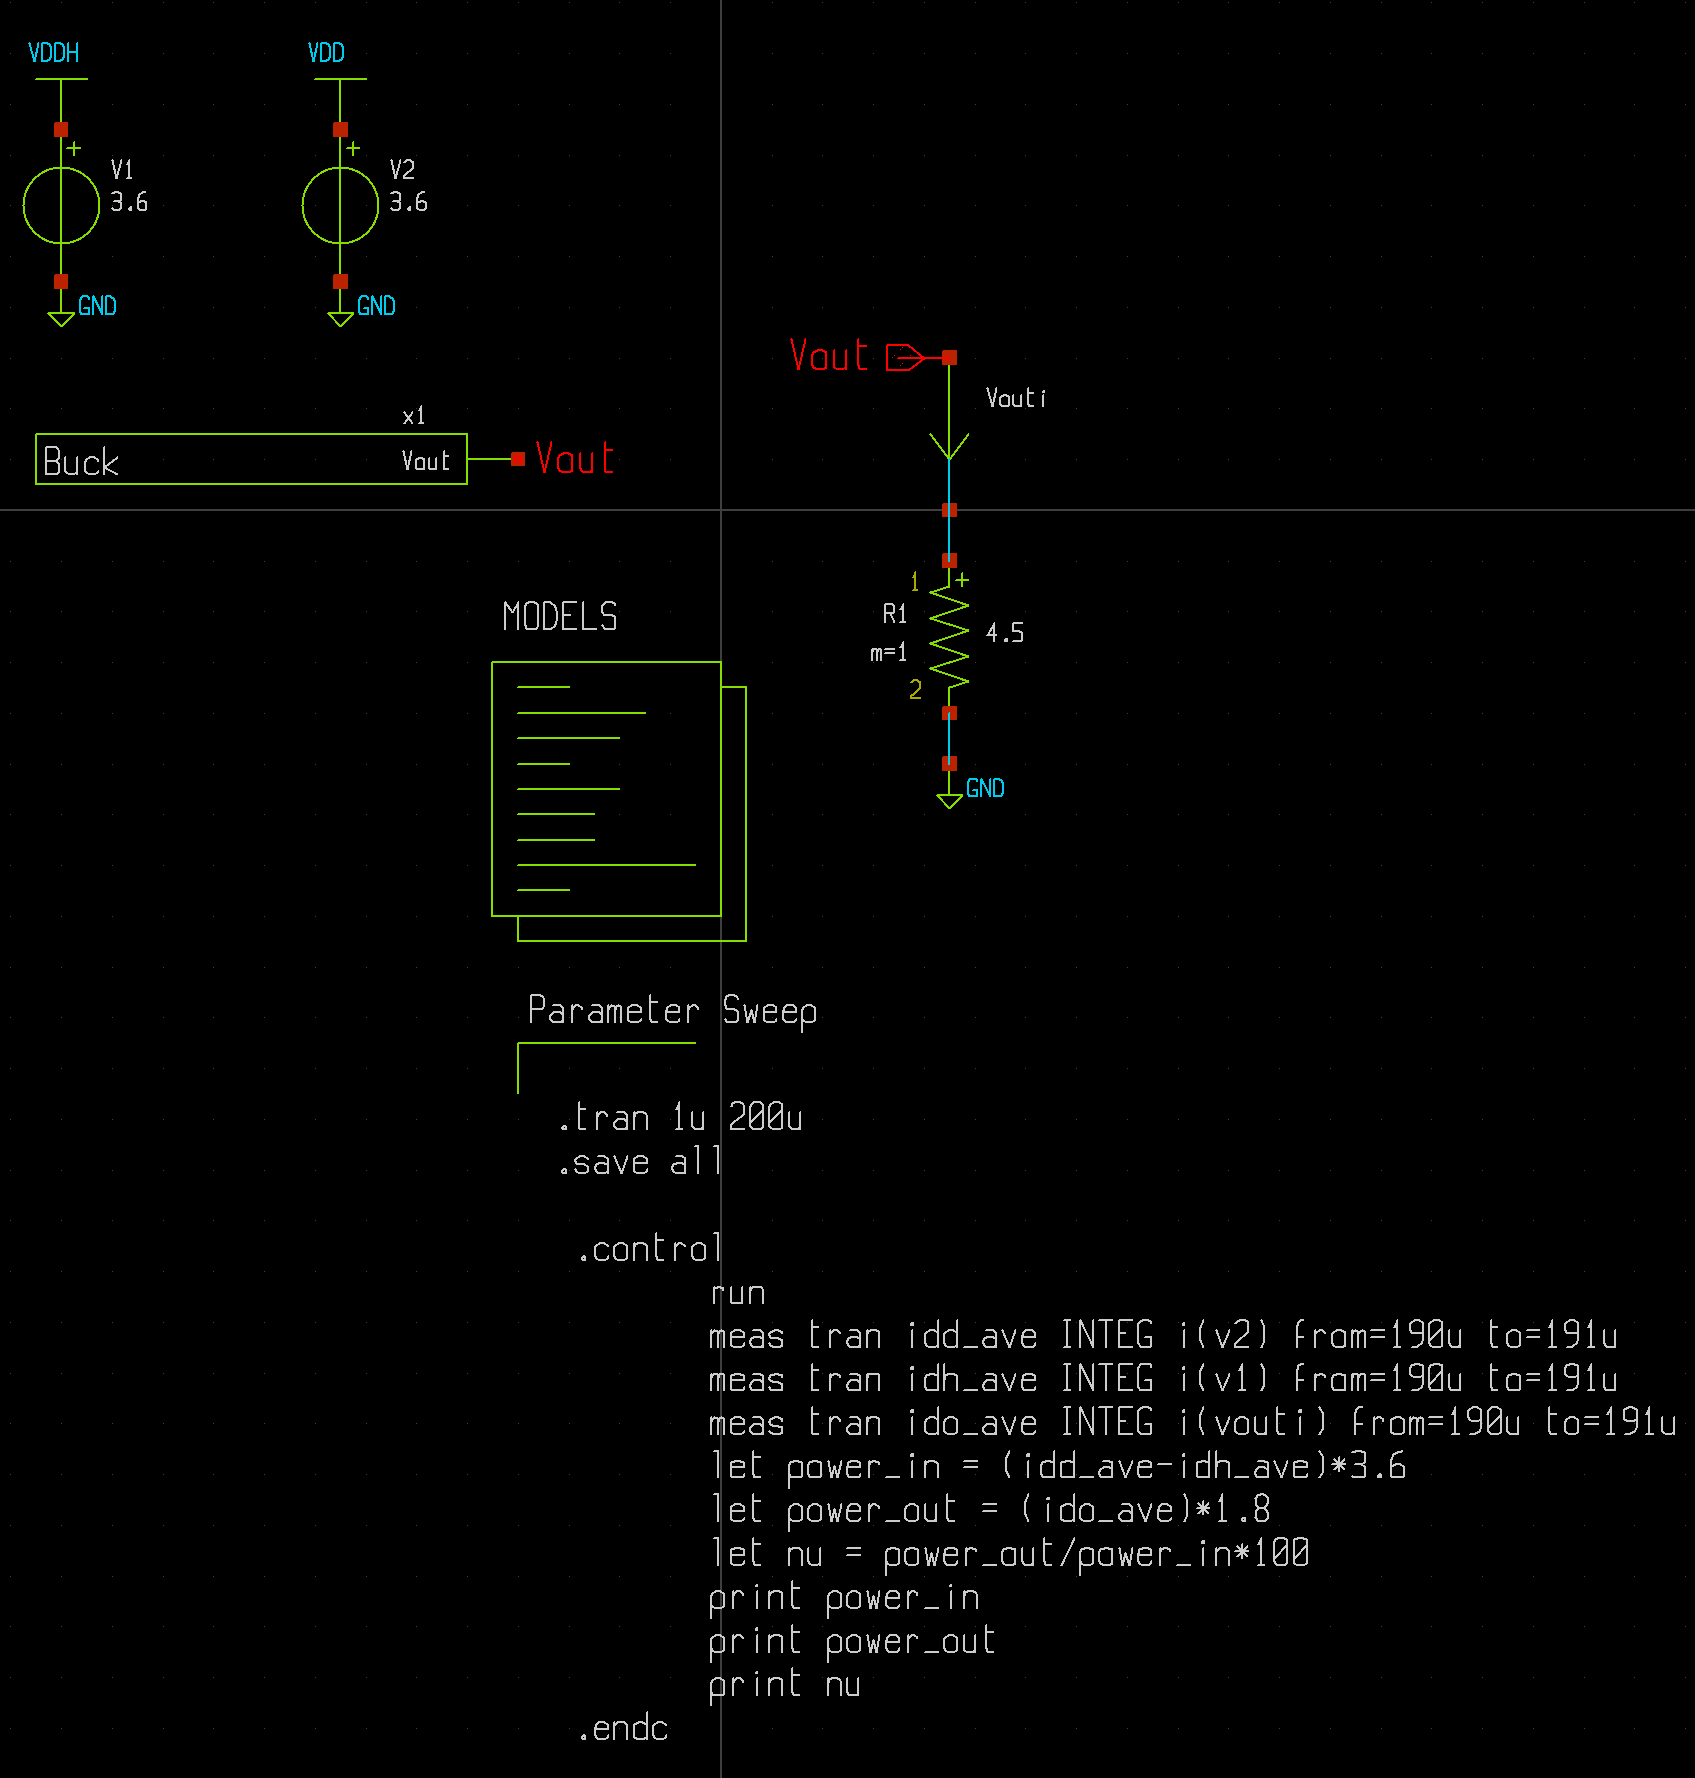
\includegraphics[scale=0.10]{testbench.png}
\end{frame}

\begin{frame}
  \frametitle{Vout at Startup }
  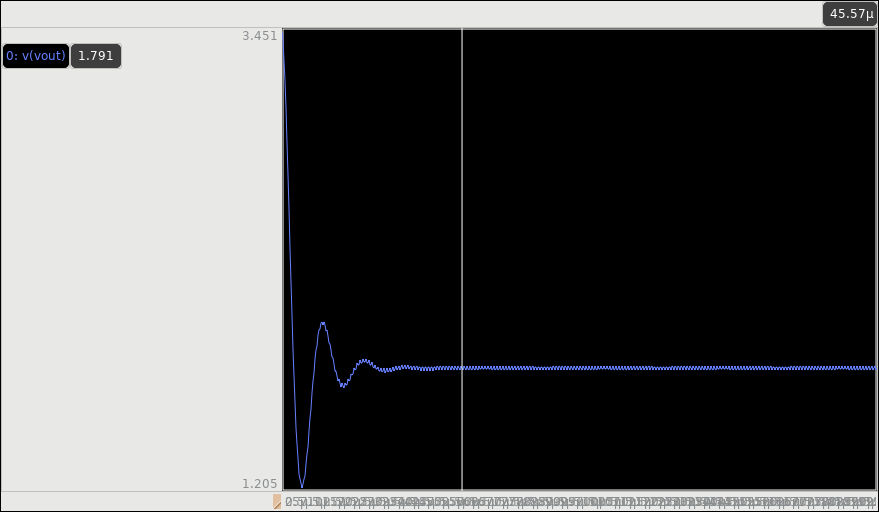
\includegraphics[scale=0.25]{startup-to-steady.png}
\end{frame}

\begin{frame}
  \frametitle{Ripple}
  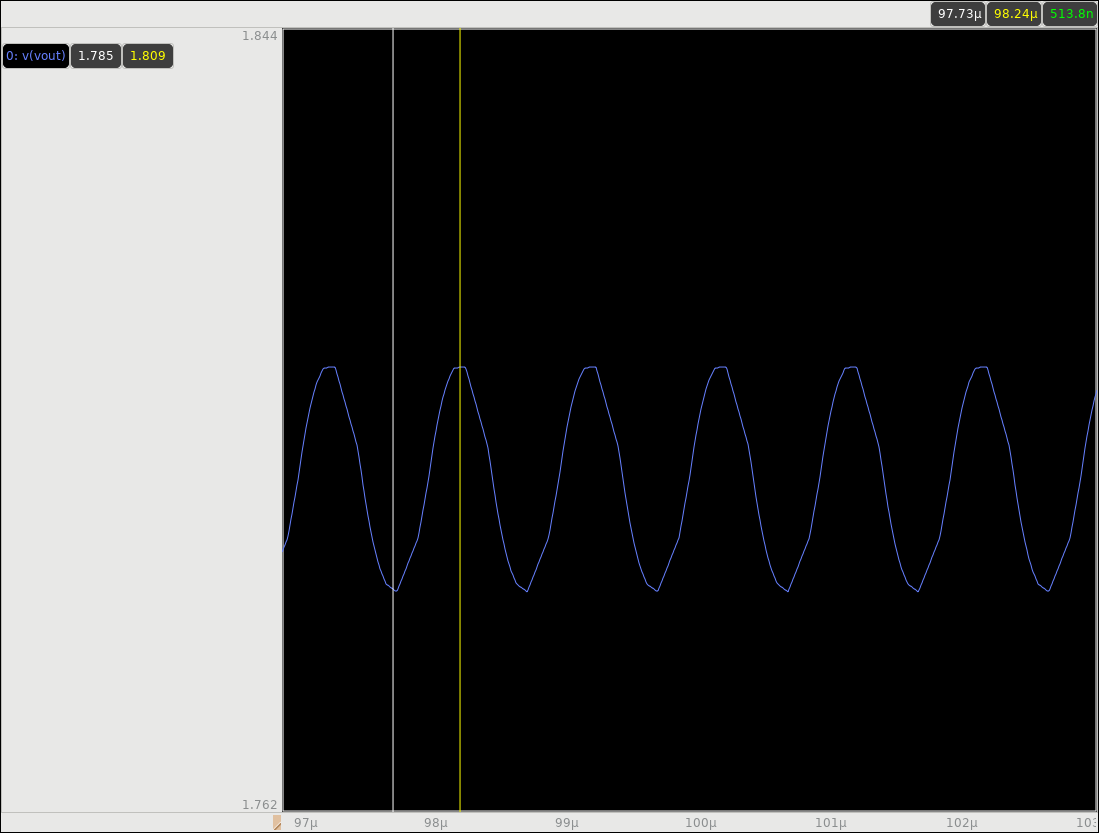
\includegraphics[scale=0.25]{ripple.png}
\end{frame}

\begin{frame}
  \frametitle{PWM input and Deadtime output at $Vin = 3.6V$}
  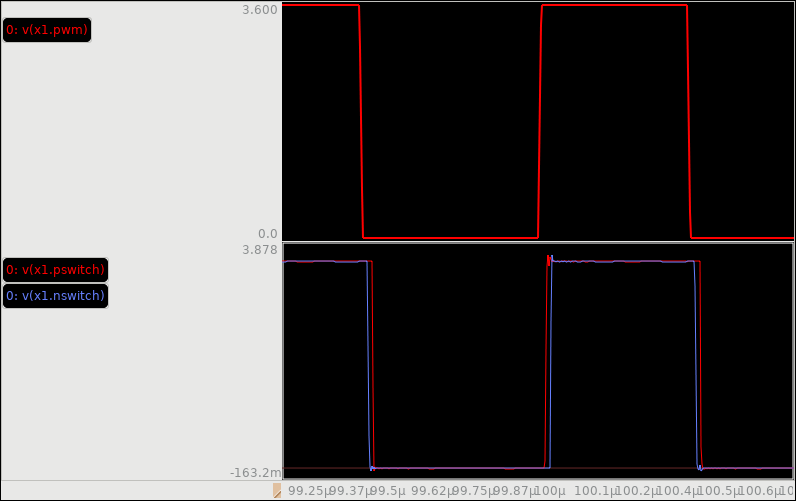
\includegraphics[scale=0.25]{pwm-deadtime.png}
\end{frame}

\begin{frame}
  \frametitle{Deadtime Measurement at $Vin = 3.6V$}
  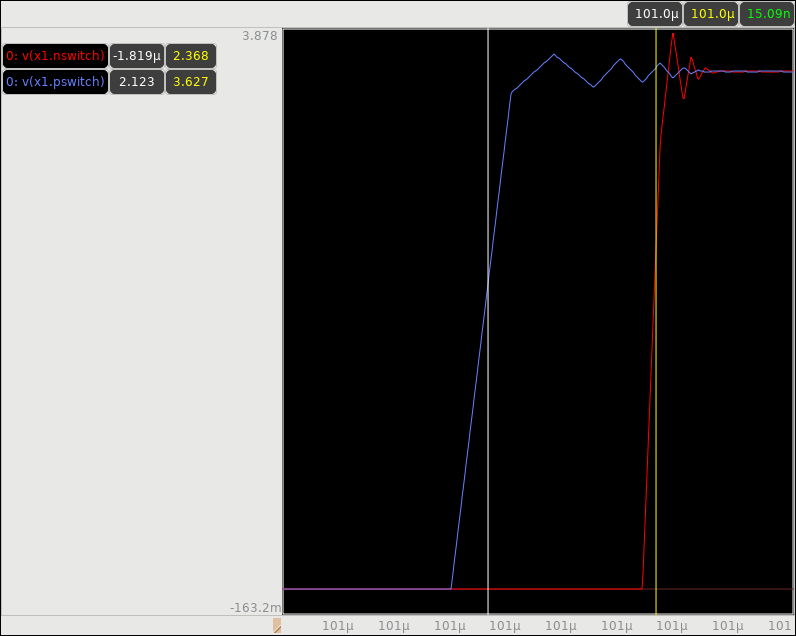
\includegraphics[scale=0.25]{pwm-deadtime-rise.png}
\end{frame}

\begin{frame}
  \frametitle{Drive Train Output $Vin = 3.6V$}
  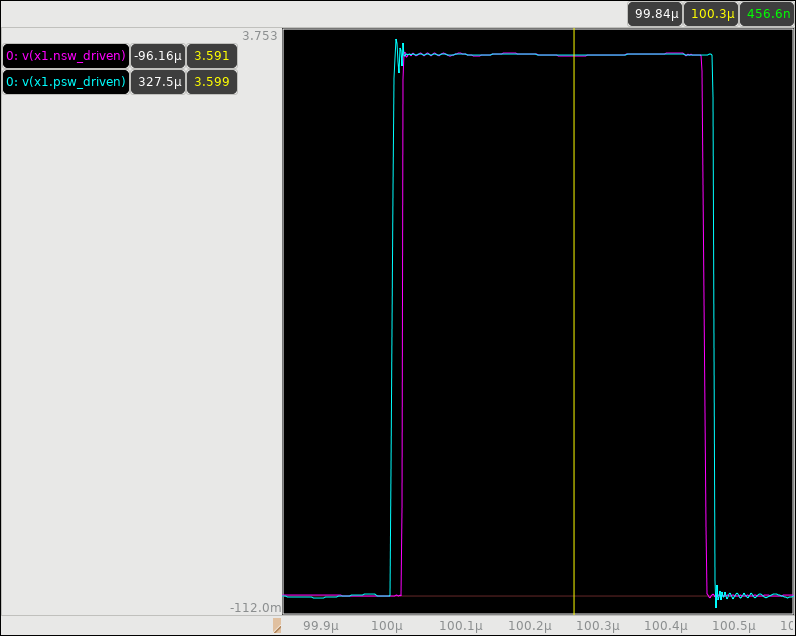
\includegraphics[scale=0.25]{drive-train-output.png}
\end{frame}

\begin{frame}
  \frametitle{Power FET Currents}
  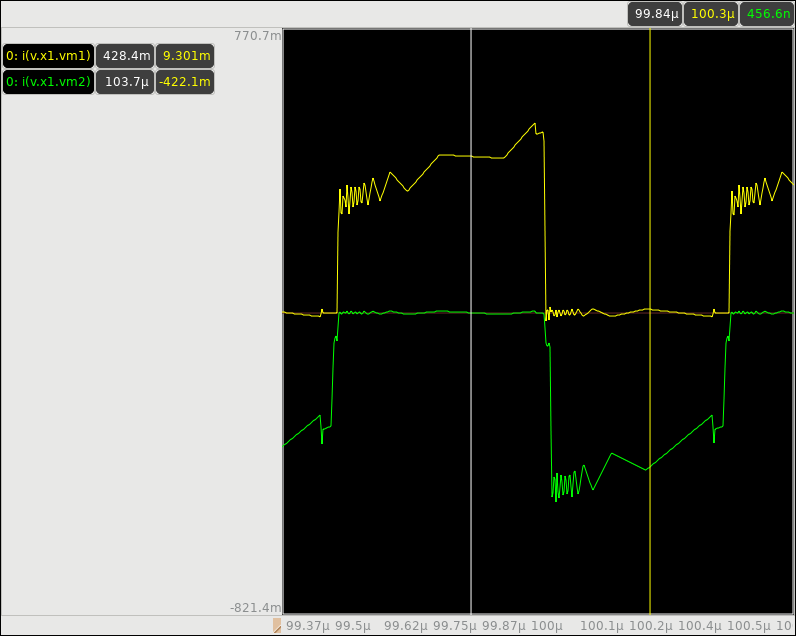
\includegraphics[scale=0.25]{hiside-lowside-current.png}
\end{frame}


\begin{frame}
  \frametitle{Efficiency}
\end{frame}


\end{document}
